\documentclass[../main.tex]{subfiles}

\begin{document}
\chapter{Position finding solutions and applications}
* What features should have the model in order to be used for navigation?


\section{Known solutions analysis}
%Known solutions analysis (against defined criteria)
\begin{itemize}
	\item List of known positioning system in underground installations
	\item Characteristics of known positioning systems
	\begin{itemize}
		\item Their concept Advantages and disadvantages
		\item How can be used
		\item How they perform the communication (physic/hardware aspect)
	\end{itemize}
\end{itemize}

There are known solutions for location and monitoring people in undergorund installations. They are together named as LAMPS systems - Location and Moinitoring for Personal Safety systems. Those systems use three components in general:
*


Positioning systems with respect of the what is the target of acquired data. There can be defined three categories of positioning systems: positioning systems that are dedicated to acquire and transfer information about objects position to systems on surface, systems that are dedicated for on site usage to locate the device inside the underground installation and systems that combine both approaches.


Computer recognise loading and dumping points by data provided by positioning system. It acumulates data about machine speed, distance traveled, time, amount of load that is carring and put into the report which creation is triggered by positioning information.


\begin{itemize}
	\item Advantages and disadvantages of solutions
	\item How the solutions fulfil given criteria (ex. how accurate given solution can be)
\end{itemize}

Possible subsections that will discuss in detail given technologies.
Inertial system
https://en.wikipedia.org/wiki/Inertial_navigation_system

Considering reference points:
\begin{itemize}
	\item communication technology:
	\begin{itemize}
		\item Bluetooth - the availability, supported by modern mobile technology,
		\item ZigBee,
		\item WiFi
		\item RFID
		\item ... others
	\end{itemize}
	\item system architecture
	\begin{itemize}
		\item server - client
		\item client - server
		\item WSN and IOT
		\item Peer-to-Peer
		%[Felix C. P. Hui, Henry C. B. Chan, and S. H. Fung. RFID-based Location Tracking System Using a Peer-to-Peer Network Architecture[J]. Lecture Notes in Engineering & Computer Science, 2014,2209(1):135-140.]
		%\item With respect of where environment layout model is stored (related - GIS systems; GeoSoft, Vulcan, MineSight, SURPAC Range, or Mining Visualization System (MVS))
	\end{itemize}
\end{itemize}

%WIRELESS TECHNOLOGIES

%BLE
%ZigBee

\subsection{WiFi signal strength analysis and WiFi fingerprinting} % (fold)
\label{sub:wifi_fingerprinting}

WiFi network infrastructure is a one of the available solutions that can be used as a source of information about current position of the device. The basic solution for positioning with use of this technology is about recognising wireless lan network access points by thier SSID or physical address of network cards \cite{WLAN_fingerprinting}. As there exists working position finding solution that base on that technology the accuracy of the solution is about 100-300 meters \cite{thesis_tablet_positioning}.

What is specific for radio waves attenuation at 2,4 GHz frequency is that their signal is present from relative large distances in mine in compare to the same devices signal range in the open space environment. What is also characteristic is that the signal strength, after its peak close to the WiFi transceiver antenna its going to stabilize in distance about 10m from source and then the signal strength is residing on similiar level up to distance arround 300 meters from its source when it goes down \cite{Thesis_CM}.

\begin{figure}[ht]
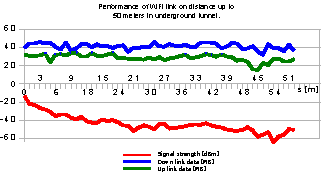
\includegraphics[width=\textwidth]{pictures/wifi_link_short.pdf}
\centering
\caption{Wireless lan throughput and signal strength with respect of distance from the signal source (wireless access point) \cite{Thesis_CM}. }
\label{fig:wifi_link_short}
\end{figure}


On figure \ref{fig:wifi_link_short} it is presented how wireless lan link parameters differs with respect of distance between client device and the network access point. Measures presented there are taken from 0 up to 50 meters from signal source. In case of this chart there were presented uplink and downlink throughput measured by amount of data gathered on each testing probe taken each meter distance from the signal source and the related signal strength expressed in dBm units. Values presented on chart are medians of all gathered values and factors for given distance. Test was caried out in straight underground tunnel in the biggest coal mine in Slovenia: Premogovnik Velenje. Connection throughtput between client and server remains nearly the same for distances in range from 0 up to 50 meters. Signal strength is presented in logarithimc unit dBm. Signal strength falls significantly in first 10 meters from 0 to -40 dBm. After distance of 10 meteres value of signal strength is ranged in between -40 and -50 dBm with small and not regular diviations. After 45 meters from source the value drops slightly bellow -50 dBm.

\begin{figure}[ht]
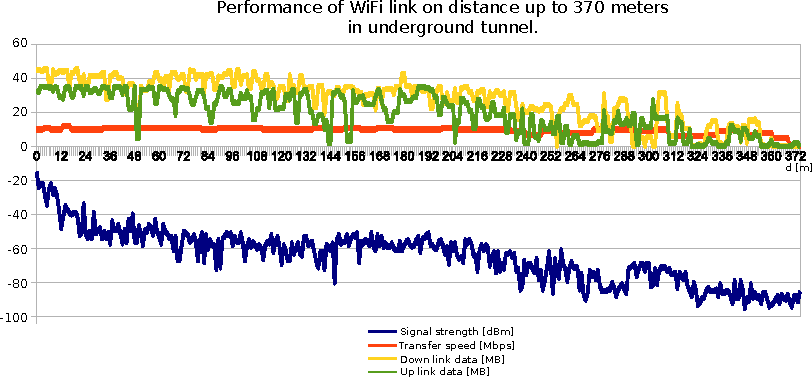
\includegraphics[width=\textwidth]{pictures/wifi_link_long.pdf}
\centering
\caption{Wireless lan range \cite{Thesis_CM}. }
\label{fig:wifi_link_long}
\end{figure}

Figure \ref{fig:wifi_link_long} presents tests results performed on longer distance till connvectivity was not possible due to too low signal strength. On distances from 50 up to 240 meters parameters of link are similiar. Down link data remains at 40 MB and at 38 after 140 meters with drops to 20 MB. Up link data measurments are more unstable than in case of down link in therms of drops in delivered amount of data, but trend seems to be steady on range from 50 till 220 meters from access point. Then both data uplink and down link drops by 10 MB.  Speed of data transfer between access point and client device remain similiar from very beggining till distance around 370 where signal is not enogh to conduct connection. Signal strength is characteristic only for first 10 meters from signal source. Then signal strength oscilates between -40 and -60 dBm on distances 10 -- 50 meters, between -50 and -80 dBm on distances 50 -- 240 meters, between -60 and -90 on distances 240 -- 320 meres and between -80 and -90 on longer distances. Following data does not represent any straight forward solution to adjust positioniong information to make positioning more precise and accurate. Only on distances close to the signal source it is possible to estimate more precise position while signal strength values differ significantly from the values that occures on the rest of distances. There can be identified following range zones with respect of WiFi signal behaviour \cite{Thesis_CM}:
\begin{enumerate}
	\item near field zone: 0 -- 40m distance from signal source where wave attenuation curve is similiar to that in free field distribution,
	\item coverage zone: 40 -- 200m distance from signals source where can be identified symptoms of waveguide propagation and signal strength remain to be arround -50 dBm,
	\item monitoring zone: distances since 200m from signals source where signal starts to vary from -75 up to -85 dBm and becomes to be unusable for communication purpose but client and access point are visible for each other,
	\item out-of-range zone: where signal is too low and both client and access point are not visible for each other.
\end{enumerate}

One of the approaches for the Wireless LAN based positioniong system is to assume that given client is present in given area of underground installation if it is in coverage zone of one of Wireless LAN access point. Client can be registered by access point software and followed until he leave coverage zone. As the coverage zone is about 200 meter distance from access point then total accuracy of this solution is about 400 meters. Second approach assume positioning accuracy improvment by signal strength interpretation and recognistion if client is in near field zone. This approach is easy to be implemented as signal strength values in near field zone differs from values from the rest of zones. Such solutions are implemented in mines in Germany \cite{Thesis_CM} and in Swedish Boliden's mines \cite{thesis_tablet_positioning}.


%TODO - wlan and AoA; wlan and ...???
%TODO - fingerprinting; There is known concept of recognising position in mine by informations distributed by


% subsection wifi_fingerprinting (end)

\section{Positioning with Beacons and Bluetooth technology} % (fold)
\label{sec:positioning_with_beacons_and_bluetooth_technology}

Beacons are transmitters that use Bluetooth low energy technology in order to send out small set of informations. They are designed to be small and energy efficient in order to allow them to be independent from the external power source. The main application of beacons are indoor positioning systems while beacons can be treated as a set of reference points building the static infrastructe of landmarks where the position is a funtion of received signal strength from beacons by the user. Beacons can be also attached to the non static objects or even user can emmit beacon information. Then the responsibility of position estimation lies on the infrastructure that gathers the signals.

Common way of estimating the position is taking into account the measure of received signal strength from the beacon transmitter called RSSI (received signal strength indicator). RSSI denotes the power of received radio signal measured in dBm (decibel-miliwatts). The measure is actually the raw value that express the powerd inducted on the receivers antenna as a result of transmission. None additional sensors are required to take that measure. Value is available on most of wireless technologies as a part of diagnotic report serving as indicator how good the connection is. The higher the RSSI value then the higher the signal strength so transmitter is closer to the receiver. Such relation between the RSSI value and the distance is known under a various of models that tries to describe the propagation of electromagnetic radio waves with use of some statisic and probabilitic distribution \cite{RSSI_path_loss_prediction_model}. Such models are needed because of calculus complexity while using actual physical model of the phenomena. In order to perform physical calculus there is need detailed description of the envioronment including every element that may influance the radio wave propagation. Calculus could include d'Alembert equation for signal power density on limited space which requires 6 variables concerning distance and time in 3 axis. Calculus should take into account presence of radio wave diffractions and attenuations on materials present in the indoor envioronment. As the propagation space is not ideal and the amount of elements influences the propagation is large such calculations are not being performed.

Example of statisically obtained model that descibes relation between received signal strength is \textit{Log-distance path loss model}:

$$ RSSI = -10 n \log_{10} (\frac{d}{d_0}) + A_0 $$

where $ d $ is the distance between the receiver and transmitter, $A_0$ is a reference RSSI value measured at $d_0$ distance from the transmitter, $n$ is the signal propagation exponent. Taking the measure of RSSI ($A_0$) at a distance of one meter from the signal source ($d_0 = 1$) simplifies the equation. That is the common practise which was even implemented into iBeacon protocol developed by Apple company by attaching additional information about reference $A_0$ RSSI value into the broadcast message of the beacon.

\textit{Log-distance path loss model} states that the only variable that influence the RSSI value is the distance from the source. Such model has to treaten as a rough distance estimation as RSSI is not a stable measure. Bluetooth technology operates on a 2,4GHz frequency which means that the wavelength of the signal is equal to 12,5 cm. Such short wavelength is prone to distrortion such as multi-path reflections where signal bounce against objects and material attenuation what makes the resultant measures noisy.

Bluetooth technology was developed and is maintened by the Bluetooth Special Interest Group (Bluetooth SIG) which is the standard organisation capable for licensing the Bluetooth technologies and trademarks to the manufacturers. Bluetooth technology operates on frequencies from 2,4GHz to 2,4835GHZ which was devided into into 80 channels. In order to adopt transmission channel to the current load on given frequencies, Bluetooth implement a mechanism called \textit{Adaptive Frequency Hopping} which allows to change channels being in use during the transmission without interrupting it. Subsequent Bluetooth technologies are aimed to ensure bigger data transfer, lower energy use and increase the transmission security. Since version 4.0 if Bluetooth standard there is availablable special protocol that is optimised for lower power consumption. This protocol is called \textit{Bluetooth Low Energy} while the whole Bluetooth 4.0 standard including classic and high speed protocols is called \textit{Bluetooth Smart}. Since 5.0 version of the standard the set of the protocols are called just \textit{Bluetooth 5}. Market is dominated with Beacons that use Bluetooth Low Energy protocol in version 4.0 that is why this paper focuses only on this version of protocol.

Bluetooth is as set of profiles. Each version of the technology contain definitions of profiles that are up to date to that version and optionally are reverse compatible with older ones. Each profile describe what communication protocols and data format it use. Protocols available for the profiles are also defined by the Bluetooth technology. Bluetooth Low Energy protocol use \textit{Generic Attribute Profile (GATT)} which is a set of services that can be used within the transaction between devices. Service is a name for collection of characteristics that express state of device. Bluetooth defines 59 services within the GATT such as TPS (Tx Power Service), IPS (Indoor Positioning Service) or HRS (Heart Rate Service). Services are idenfied by their UUID number which must be unique. Despite the defined service, there is a possibility to create own services. Characteristics are defined with given format type, properties and security permissions. There are available such format types as signed or unsigned integer ranging between 1 and 8 bytes, float, string or a structure. Allowed properties of the characteristics describe if the value within the characterisic can be readed (read property), changed (write property), required acknowledgement (indicate property) or being in use just for notification purposes (notify property). There is possibility to add custom properties as well. Security persmissions part of the characteristic definition are about definining if given property can be executed with or without an authentication. For example Measurement Interval characteristic of the Health Thermometer Service is defined with Read, Indicate and Write properties and security permissions stating that there is not required any authentication for reading but it is needed for writing.

Broadcast messages are way how Bluetooth Low Energy devices communicate with them selves. In order to distinguish types of messages they use different format of this message. On the market of Beacons there are two major protocols that defines broadcast message format. The first -- \textit{iBeacon} -- was developed by Apple and the second -- \textit{Eddystone} -- was developed by Google. Those broadcast messages formats are the basis for creating "Ranges" definitions explained in details in section \ref{subs:smartphone_abilities_and_limitations}.

% section positioning_with_beacons_and_bluetooth_technology (end)

\subsection{RFID tags} % (fold)
\label{sub:rfid_tags}

RFID technology make use of electromagnetic field phenomena that allows to transfer information to reader from special component, RFID tag. Passive RFID tags are powered by readers though electromagnetic field; they do not use batteries or wired external supply. In order to acquire information from tag readers have to propagate electromagnetic waves. Tags cumulates power from electromagnetic field in capacitor. When tag have enough power then it transmits the response with tag's data to the reader and goes to sleep for a given time. Reader get signal from tag and perform filtering and decoding operations on it in order to get tag's data. There are also available variants of active RFID tags wich use it's own power supply.

RFID technology is used in underground installations in certain locations to serve as check points. In this manner are monitored underground trains or dispatch of materials is being monitored. Passive RFID modules are installed on containers or mobile machines like trains. Those modules can be read by passive RFID readers that are connected to the mine network via dedicated control unit like Mining Infrastructure Computer \cite{Thesis_CM}. Control unit is responsible for RFID reader configuration and translation of its readings into standarized positioning information format. It also supplement data from RFID reader with its identificator or coordinates which express position of a reader on mine model. RFID can operate at 868MHz band. RFID with 8dBi antenna is able to detect RFID passive tags at range of up to 3 meters.

%WHAT IS THE RANGE? HOW MANY ENERGY MUST BE USED TO GET THE DATA FROM RFID?
% subsection rfid_tags (end)


\subsection{WSN based position finding systems} % (fold)
\label{sub:wsn_based_position_finding_systems}

There are proposals of position finiding and tracking systems based internet of things (IOT) soultions \cite{WSN_tracking, WSN_monitoring}. The idea is to create means of wireless communication to locate miners during their daily basis. It is proposed to create a network of wireless nodes (WSN) that read signal from tag devices (RFID) carried by miners and transfer it through nodes network to sink nodes that are directly connected to the mine core data transfer installation such as industrial Ethernet. Miners position data is sent to acquisition server. Intermediate and nodes are directly connected one or more nodes laying in the range of their wireless communication module. They form together ad hoc, multi-hop, self-organizing network of nodes that is able to transfer data, reorganise its structure in case of mailfunction of one of the nodes and allow to configure nodes remotely due to the implemented wireless communication technology and dedicated routing protocol. Network of nodes can be easily expanded by adding new nodes. Due to the fact that communication is wireless, nodes can be placed also in danger or new areas where wired network devices are not allowed or the related infrastructure doesn't exists.


WSN and RFID based positioning system is designed to serve such functionalities as querying miner information, locating miner, tracking miner and managing tag and reader. It is proposed to use this system along with simillary implemented monitoring system that measure safety parameters in mine \cite{WSN_monitoring}. This positioning system is dedicated to used by production monitoring, production scheduling and emergency rescue mine departments located on surface. Bigger precision can achived by adding more nodes into the network. Technology that is used for wireless communication between WSN nodes can be a Bluetooth Low Energy, ZigBee (IEEE 802.15.4 based) or WiFi (IEEE 802.11). ZigBee technology is the most popular in WSN's as it supports variety of communication modes, contain out-of-box solutions for network topology management and support low energy solutions like sleep modes \cite{ZigBee_applications}. ZigBee protocol which is dedicated for ZigBee technology uses energy and computational efficient solutions for data collision avoidance which includes CSMA/CA techniques and time division concept \cite{WSN_monitoring, ZigBee_desc}. There are three main topologies forced by ZigBee technology that can be used in the WSN network: star topology, tree topology and mesh topology. Star topology limits the network to have all nodes directly connected to sink. Tree topology enables multihop functionalities but litmits network flexibility in therms of adopting routes in case of filure (doesn't support redundant connections between nodes). Mesh topology requires to store routing tables in each node but provides means of redundancy in therms of routing what makes the WSN network reliable and fault resistant \cite{ZigBee_desc}. The WSN positioning network proposal base on ZigBee technology and it's mesh topology. Placement of WSN nodes should guarantee signal coverage of RFID readers modules build into nodes. On order to achive that there are proposed variety of topologies that can be used on site during network installation. On image \ref{fig:wsn_topology} it is presented the network topology proposal that introduces intermediate nodes -- routing nodes -- that gather information from sensor nodes and transfer it through network of routing nodes to server via sink node \cite{WSN_monitoring}.  Due to the fact that WSN nodes are limited in energy supply, systems that base on that technology needs to be designed with aware of energy management and fault management. Idea of routing nodes deployment along the tunnel in two simmetrical lines comes from the need of link redundancy between nodes. Thanks to that even if some of routing nodes are down the information from sensors can be passed out through the other routing nodes that are in range. In order to limit power consumtion of reader nodes they were designed as Reduced Function Devices (RFD). These nodes do not take a part within information passing process. Reader nodes are designed only in purpose of reading signals from RFID tags and to send the information to the nearest routing node. In order to achive that the information will be sent only to the nearest reouting node there is performed initial configuration process that involve both reader nodes and route nodes in its signal propagation range. The process is such: reader node send the testing signal to all of the nodes. Nodes that were able to reiceve the signal, send responce with value of Received Signal Strength Indication (RSSI). Reader node limit its sending power according to the responces. Thanks to it power consumtion of reader node and interference with neighboring nodes are reduced.
%WHAT IS THE PRECISION? HOW CAN BE APPLIED INTO MOBILE PHONE (TARGET)? WHAT IS NODES POWER SUPPLY?

\begin{figure}[ht]
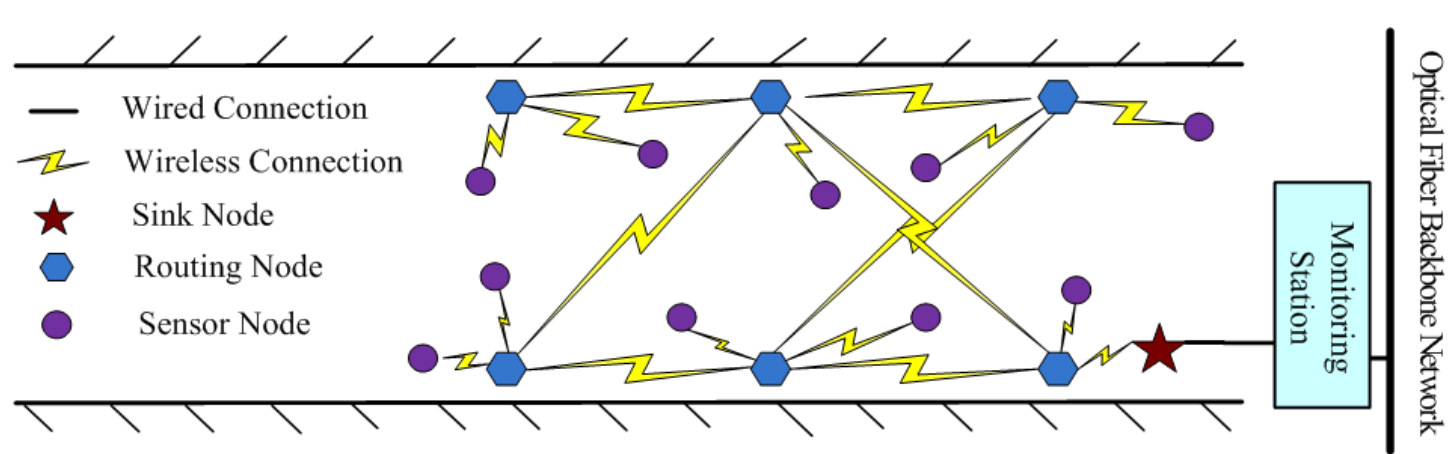
\includegraphics[width=0.7\textwidth]{pictures/wsn_topology.png}
\centering
\caption{Wireless Network Sensor topology in underground corridor example \cite{WSN_monitoring}. }
\label{fig:wsn_topology}
\end{figure}

%WSN routing and topology
Network of wireless connected nodes needs be designed with respect of its maintability. There is need to assume that some nodes may fail during their operation. As the network consits of many nodes, where the number of nodes can be changed during thier operation, there is need to implement actions that will allow them to organize their topology automatically. Even if particural nodes will fail, the rest of nodes should be able to work and maintain communication with remote services. It is the role of implemented routing protocol. There are available solutions that allow network to adapt quickly to the changing environment \cite{WSN_collective}, but in case of statically placed network elements the environment is not changing havily. As it is in common practise, routing nodes stores information about nodes that are used for network purposes in the routing tables. Rounting tables are created with the manner that there are promoted link to nodes that ensure the lowest cost (distance) of packet travel from given node to the sink node. Routing table can have many entries. In case of topology for underground installation there are suggested 3 entries: parent route, minimum route, backup route \cite{WSN_monitoring}. Parent route points to the parent node, minimum route points to the best node in therms of the most energy efficient way to the sink node and backup node that points to the second to the best routing node. Each entry consists of elements such as: number of hops (routing nodes from itself to the sink node), value expressing quality of link of the last communication, flag that describe the role of the entry (parent, minimum, backup route). Routing tables and interconnections between nodes are created during network installation process. The idea is that the sink node that is directly connected to external communication medium creates at first 1-node WSN. Rest of nodes organize themselves in manner that nodes broadcasts their physical and network adresses. Basing on information gathered during installation they are able to determine their position in the network, obtain network address, assign routing table entries and obtain hop number. The network topology can be build up and maintain after WSN installation process \cite{ZigBee_applications}. Nodes are able to pass information to sink node that contains it's routing tables. Thanks to that sink node is able to recreate network topology and then pass the information to the external server. In order to maintain the network there are implemented status messages that contain information about changes in nodes routing tables. They are usually pass through WSN along with data from periodic sensor readings.

%WSN power management
Nodes are equiped with batteries that makes them independent from external power source. In order to save the energy and in order to prolong device live on the battery nodes works in energy efficient modes. In these modes nodes are turned into sleep for certain time. They woke up in order to perform tag readings and transfer the data to the external resources. In order to synchronize their operation, in each cycle the sink node broadcasts the initial message which is used to synchronize all of attached nodes. Power level of nodes batteries are monitored. Nodes can send information about their power level as a repsponce for appropriate request. There can be implemented special routines inside node that can cause sending the information about the low battery level in emergency mode, without any request from the sink node.

%WSN Location management
The crucial for the positioning system is to determine accurately exact position of given reader node inside the underground installations. Without information about readers placement positioning data obtained from them are not usefull. Solution for this problem in WSN positioning systems are solved by manual configuration. Each node have it's own identification number that is a part of it's initial configuration. This number is atteched into their housing also so given nodes can be identified directly during the installation or maintenance work in tunnel. As nodes deployment is regular it is assument in advance what will be the position of the node within the tunnel. In case of sudden failure of some node it is possible to determinate which of the node is broken by it's ID information, and check were the node is placed. WSN network should have possibility to report failure of its nodes. That is why WSN positioning systems are equiped with failure detection and reporting mechanism. Parent nodes like routing nodes against reader nodes, checks if child nodes responds to the requests. In case of having no response from given node for a given amount of subsequent requests then parent node issue status request command to the child node and wait given amount of time. If child node give an answer then it is assumed that the given child node is working correctly. In case of no response from child node, the parent node send information about failure to external service. As the readers nodes are connected stright to the parent node with no routing options then different policy for borken parent node must be applied. If the child node does not reiceve acknowledgement (ACK) frame from it's parent given amount of times then the node increase it's sending power and retrainsmits it's data again. If there is no result of increasing the power then node goes into network setup mode and scan channel to rejoin the network.

%General solution Architecture
Positioning algorithm in WSN positioning system base on mine layout and assume fixed position of nodes. Information about mine layout and nodes position wihin mine is stored in database on server above ground. Data transferred from nodes into acquisition server is a combination of three values: ID of a node, ID of acquried RFID tag in range of RFID reader module of that node, signal power of this RFID tag, and timestamp. Data is being stored in simplified relational database. This positioning system uses algorithm for finding exact position of RFID tag in dwo diamensional space (x, y). In order to do that algorithm search in database for 3 nodes that acquired given tag sinal with the biggest power. Then it uses simple free space electromagnetic waves propagation model \eqref{eq:prop} to compute distance between node and tag.

\begin{equation}
\label{eq:prop}
P_{ri}=\frac{P_t \cdot G_t \cdot G_{ri} \cdot \lambda^2}{4\pi D_i^2}
\end{equation}

Parameters $P_t$ (signal power generated by tag), $G_t$ (tag antenna gain), $G_{ri}$ (node reader antenna gain) and $\lambda$ (electromagnetic wave length) are constant and known. Parameter ${P_{ri}}$ (received signal power on reader's input) is the only variable in the equation that is needed to compute distance from tag to reader. Maximum likelihood estimation method that base on data from three nodes and thier values of reiceved signal power from given tag produces relative position of given tag in (x, y) coordinates. Suggested implementation \cite{WSN_tracking} assume that nodes look for RFID nodes each 10 minutes.
% subsubsection wsn_based_positioning_finding_systems (end)

%drawback of WSN - simplified assumtion about propagation in underground corridors because of wave diffractions on it's walls; - not needed precision of two diamensional space; assumption about RFID tag range (WHAT IS THE RANGE OF RFID). In order to fulfill assumption there is need to put WSN nodes close to each other which higher the costs; - Limited lifetime
%advantages of WSN - wireless nodes with rfid reader modules are cheaper than wired ones (in the same price we can install more nodes)

\section{Mobile device dedicated positioning systems} % (fold)
\label{sec:mobile_device_dedicated_positioning_systems}

Todays smartphone class mobile device contains set of sensorics that can be used as a base for interial positioning system. In underground oprations industry this idea is not the newest as there were tryies of this technology implementations inside handheld devices for people working underground with use of semiconductor based MEMS gyroscopes \cite{Thesis_CM}. Such devices were connected to the underground wireless network through access points which was responsible for transfering positioning information to the central systems above ground.

Smartphone class devices contains set of components that are treated as common in the industry. There is no strict definition what components should or should not the smartphone class mobile device contain as there is a strong competition in the market offering those devices in various configurations, shapes and fetures. This paper focus on devices that are compliant with Android operating system, especially version 7.0 which is currently (in the middle of 2018), the most popular operating system on the market. TODO - reference needed - TODO. Android operating system forces hardware manufactures to equip devices with at least a minimal set of components needed for the system normal operation and give recommendations of optional components that are natively supported by the system  - TODO - take from Android 7.0 Compatibility Definition - TODO. In this section there will be investigated only those technologies that are available for the basic handheld mobile device with Android 7.0.

Smartphone class mobile devices are treated in the engeener industry as a powerfull tool set helping the workers with their maintenance work on site and as a handy platform for wide scale of businesss oriented applications for task management and reporting. Factors that attract potential users of such smartphone based solutions are mainly connected with the price of those devices, ease of use, well described and supported programming frameworks and IDE, ready to use libraries, solved main power management and security issues, ease of maintenance, modularity, scalability, support for the most popular data exchange technologies, ease of extending the functionality by adding the support for external, wireless equipment. Smartphones that are available in the market are also equiped with the sensorics that allow the users to detect, record and recognise the phisical movements or orientation changes. It extends the positioning functionality making it more robust and acurate.
% section mobile_device_dedicated_positioning_systems (end)

\subsection{Mobile device sensorics}

There is no limitation in extending smartphones with internal sensorics. Acording to the Android 7.0 Compatibility Definition - TODO - there is no such sensoric that must be mounted and implemented into the Android system in order to be compatible with the operating system. It is also stated that device can contain as many various sensorics as producer wish under condition of having a compliant software implementation that deals with the sensorics. Although Android compatibility definition recognise some of them and recommends to be installed on the device. There are also technical requirements given under the sensorics recommendation in case of presence of such on the device.

In sake of simplicity Android defines all of componentes providing external information to the device as sensors. Thus components such as GPS signal receiver or a processed and filtered sensor fusion outcome like in case of rotation vector (fusion of accelerometer and gyroscope data) are recognised as different kinds of sensors. Such abstract definition comes from the Sensor Stack which is the part of Android framework.

Sensorics mentioned in the compatibility definition are:
\begin{itemize}
 	\item Accelerometer,
	\item Magnetometer,
	\item GPS,
	\item Gyroscope,
	\item Barometer,
	\item Thermometer,
	\item Photometer,
	\item Proximity Sensor,
	\item Fingerprint Sensor,
	\item 6-DOF Pose Sensor.
 \end{itemize}

All of components listed above, except fignerprint sensor, thermometer and photometer, can be used within the position finding system in order to give extra information about current physical state of the device. Compatibility definition guarantee some quality parameters of sensorics mounted in the mobile phone.

3-axis accelerometer can be used to detect movement changes. It provides the information how big the change was in terms of force that the device was affected. Thanks to the information there can be identified if user made a step or to compute the speed of the user in some mean of transport like a robust car by computing integral function over time from detected acceleration. It is required from that sensor to raport events at least at 100 Hz frequency (recommended minimum frequency is 200 Hz), to detect forces in range of frefall case up to forces at value of four times the gravity (4g) or more on any axis, minimal outcome resolution is 12-bits (recommended minimum is 16-bits), should allow for online calibration and calibration parameters persistance, be temperature componsated and have a standard deviation no grated than $ 0.05 \frac{m}{s^2} $. Document defines also the maximum accepted amount of power that the sensor can consume during its operation - not more than 4 mW (recommended values are bellow 2 mW during the operation and bellow 0.5 mW when the device is in static condition).

3-axis magnetometer (aka compass) provides the data concerning detected values of the magnetic field. Data available from the operating system level are expressed are in micro-Tesla($\mu T$). Sensor must be able to measure between -900 $\mu T$ and +900 $\mu T$ on each axis before saturating with the resolution of 0.6 $\mu T$ (recommended 0.2 $\mu T$ or denser). Magnetometer have to compensate hard iron and soft iron effects where hard iron offset have to be less than 700 $\mu T$. That value forces the producers to place the sensor in as far from current-induced and magnet-induced magnetic fields like speaker. Sensor installation have to support online calibration and compensation methods and store the parameters in persistent memory. It is required from the magnetometer to report at minimum frequency of 10 Hz (recommended 50 Hz).

GPS/GNSS receiver is not required component for a smartphone with Android 7.0 operating system. If the sensor is mounted then it is required to match set of time, reliability and accuracy requirements like:
\begin{itemize}
	\item Fast time to first fix requirement - sensor have to determine its position within maximum 10 secods,
	\item Accuracy and responsiveness requirement - position have to be determined at least 95\% of the time under condition of acceleration up to $ 1 \frac{m}{s^2} $, within $ 20 m $ and speed $ 0.5 \frac{m}{s} $.
	\item Robustness requitement - have to be allowed to track at least 8 satelites from one constellation simultaneusely (recommended 24 GPS satelites at the time and one from other global positioning satelite system like Glonass, Beidou or Galileo).
\end{itemize}
It is assumed that the outcome of GPS "sensor" can be supported by the information issued from the Internet such as information about current sattelites position and can be based on some assised or predicted GPS technique.

Gyroscope is an angular change sensor. If installed on the device it must be able to measure up to 1000 degree change per second, report at frequency not less than 100 Hz (recommended 200 Hz), provide information of 12-bit resolution (16-bits are recommended), be self calibrating and compensating during its work, march variance requirement defined as $ 1e^7 \frac{rad^2}{s^2} $ per 1 Hz.

Barometer is an ambient air pressure sensor. It available is must report its measures at 5 Hz frequency, be temperature compensated and have "adequate precision" for altitude estimation.

Proximity sensor gives the proximity information of an object in the same direction as the screen. The required accuracy is at least 1-bit meaning that proximity sensor produces simple outcome that is interpreted as boolean value expressed state wether the user is close to the devices screen or not.

Pose sensor with 6 degrees of freedom (6-DOF) is an optional sensor that can be implemented in the Android compatible software. Sensor provides information about himself as part of the environment in perspective of end point of maniplator with 3 kinematic pairs, each with rotation possibilities. The method and related hardware is not discussed within the operating system compliance definition. The only rescriction stated to the sensor is that it have to be more accurate than rotation vector sensor. Basic implementation can make use of camera or depth sensor to compute the output value. Output is an quaretnion that express the rotation and a translation expressed in SI units. Sensor is used in virtual reality applications.

Android compliant definition strongly recommends the procudents to provide implementations of 'composite sensors' such as step detector, significant motion detector, gravity, linear acceleration, rotation vector. These measures are an efect of digital processing of data from single sensor like accelerometer in case of step detector or a sensor fusioning basing on multiple sensors like on megnetometer and gyroscope in case of rotation vector and accelerometer and magnetometer in case of geomagnetic rotation vector. The operating system recognise already filtered and processed data directly an outcome from an composite sensor which is actually a form of abstraction that hides the details of data processing.

Management of sensorics have to be implemented in a compliant manner in order to allow the operating system to interact with those sensorics. All of the sensor outcome are yet processed, normalized and expressed in a defined way like in case of an accelerometer and magnetometer where output is expressed within the "Android sensor coordinate system" format.


\subsection{Abilities and limitations of smartphone class mobile device in context of available positioning methods}
\label{subs:smartphone_abilities_and_limitations}

In sake of generalization this paper investigate case of regular consumer grade smartphone which are devices with a common setup compliant with Android 7.0 operating system. No specialized devices are taken into consideration.

Wireless technology is a common way for exchanging the data between the handheld mobile device and the envioronment. There are available GPS, Bluetooth, WiFi and terrestrial networks(GSM related) technologies. In case of underground each of these technologies has to be installed explicitely beacause bellow the ground none of these signals are available. GNSS (Global Navigation Satelite System) signal receiver is not usefull under the ground as there is no signal from sattelites available. There are tryies to make use of that technology by re-sending the acquired GNSS positioning data from sattelites in indoor environment by a set of transmitters that mimic sattelites \cite{GPS_retransmission} but it cannot be applied to the consumer grade smartphone as the Android applications have access to already processed pseudorange data into sattelite positions. Such solution is called Glonal Navigation Satelite System based indoor positioning system (GNSS-IPS)\cite{GPS_retransmission_differential}. Approach where transmitters places on ground fake sattelite signal is known as pseudolite. In case of indoor environment positioning data acquired from sattelites are drifted due to the fact of non-line-of-sight that is why position obtained indoor is called as pseudo-position. There are known tryies of using this approach in order to obtain positioning data but there is not known any sucessful implementation in underground environment.

Terrestrial networks, like GSM, can be also used as a source of positioning information but it requires some modification in order to shortcome problems with high variance of the signal. There is no possibility to do modification on that level to the Android software on devices available on the market nevertheless some prototype installations of extended terrestial network by positioning information were done and sucessful \cite{terrestrial_positioning}\cite{terrestrial_positioning_tdoa}.

Smartphone class devices are equiped with cameras. Images that captured by the cameras can be used for positioning purposes. There are known solutions that make use of visible light \cite{visible_light_positioning} that recognise source of light like LED which are called LED beacons and compute the position basing on the angle-of-arrival (AOA) algotithm.

Thanks to the presence of intertial sensors such as accelerometers and gyroscopes there are known implementations inertial navigation. Pedestrian Dead Recokoning (PDR) is based on the measures from the accelerometer which allows for step detection and an estimation of a step length \cite{inertial_navi_unaided} \cite{inertial_navi_pocket} \cite{inertial_navi_velocity_model}. Other approaches developes the recognition patterns that allows for distiction between transportation mean being in used. Such approaches were used for example in case of prototype navigation application in Chicago, London and Cologne subway \cite{inertial_navi_subway} or inertial navigation for bikes \cite{inertial_navi_bike}. There are known solutions for interial navigation improvment by aligning the outcome to the landmarks or map information \cite{positioning_tests}.

Positioning techniques that invole following devices are not useful or cannot be connected to the mobile devices:
\begin{itemize}
	\item laser scanner as long as it requires stable position for doing the environmental mapping and recognition and it needs to explicitly be extended to some wireless communication module,
	\item ultrasonic sensor as long as it requires stable position in order to measure signal travel time correctly and needs means of computational resources in order to process the raw data and send them thorugh some wireless connection to the mobile phone.
\end{itemize}

Smartphones provides support for Beacons - simple Bluetooth Low Energy devices. There are available libraries that allows monitoring of Bluetooth devices. There are available two modes for searching for Beacons: region monitoring and ranging. Region monitoring is an energy efficient way for searching for Beacons. It allows for long delays between consequent listening periods (like 10 seconds), turning receiver into sleep mode, and background service being active while the positioning application is turned off. In case where positioning application is turned off, the background service inform user that his smartphone found himself in the range of given Beacon region and run the positioning application. Such functionality is often implemented by shopping malls official applications allowing for location aware push-messages. Such advertising technique is called \textit{geofencing} \cite{beacon_rssi_analysis}. Region monitoring gives a rough information wether there is or there is not any Beacon device being in range. On the other hand, ranging gives details about all devices being in range with details such as RSSI, name, and other, protocol dependent data. Ranging use more receiver power as listening time is bigger (like 1 second) and there are smaller time intervals between consequent listening sessions (like 10 milliseconds).

TODO - describe each of pros
TODO - describe each of cons


\begin{itemize}
	\item Which of them will be useful to increase positioning accuracy
	\item Why mobile device is good for positioning purposes? What are the factors?
	\item What means of communication (ex. wireless) can be used in context of positioning system
	\item Battery limitations
	\item Sensitivity of receivers
\end{itemize}


\subsection{Position finding basing on localization system and mobile device model}

Localization system choise (system based on beacons)
\begin{itemize}
	\item  Motivation
	\item  Prototype system description
	\item  Mobile device - system interaction description
	\begin{itemize}
		\item  Method of detecting reference points description
		\item  What are the possibilities to improve positioning on your mobile device?
		\item  How could the process of installing a localisation system in a mine look like?
		\item  How the parameters of the environment (corridor height, corridor width, type of rock, type of corridor corridors, presence of other networks operating on similar frequencies (WiFi, GSM (harmonic frequencies)), others) affect reference point signal quality.
	\end{itemize}
\end{itemize}


\section{Solution requirements}
Requirements as the position of the mobile device will be determined by the environment model.

Define criteria that will be used to compare position finding solutions (existing or conceptual):
\begin{itemize}
	\item How to save a corridor model in computer memory
	\item wireless communication
	\item resistance to power outages and communications
	\item Do I need the ability to change configuration of reference points (configuration of devices that perform role of reference points)?
	\item What parameters can be read from the reference points (range, distance, ?)
	\item How long should the network work properly?
	\item How to detect irregularities in reference points?
	\item How to fix problems in reference points?
	\item What problems may occur with points of reference?
	\item If there are restrictions upon existing network topology (ex. in order to get access to servers located on surface)
	\item Can the mobile device be useful in case of lack of signal (GSM/Wi-Fi/BLE)?
	\item example: accuracy, durability, cost, maintability (energy, fault)
\end{itemize}

Safety purpose of position finding system is very important for many countries \cite{positioning_tests}. European Union encourages to search for a good solution for the miners localization, which, in one of the postulates of its set of recommendations for the coal and steel sector ('Personnel Tracking' task). There are solutions for underground localisation but they allows only to approximate miner's position (error can be range from 300 m (range of a single radio receiver) to the distance to the next transmitter).

Underground position finding system must be compatible with mobile devices of smartphone class. Special mobile devices that were prepared to work in bad conditions like in coal or salt mines differs mainly with their housing in compare their non-commercial, personal-use equivalents. This assumption limits the range of available technologies that can be used in order to provide means of communication between mobile device and the enviornment.


Position finding system bases on idea of interaction between mobile device and the undeground envioronment. In case of the nessesity of extension that enviornment by electionic devices that will provide positioning data or means of connection with mine network there is need to state that such devices must be safe. Safety regulations in this matter differs with respect of the type of underground installation, the regional, country, or even association of countries \cite{Thesis_CM}. The goal of this paper is not to provide solution that will be adjusted to each installation type or safety regulation, but to investigate possibilities and propose state of the art solution. As the enviornmental restrictions for devices and related infrastructure that can be needed for given solution there will be assumed general rules that are being in use in commercial tunneling \cite{Thesis_CM}.



\chapter{Mobile device position finding algorithm}
* Algorithm that will make use of chosen localization system and mobile device internal sensors.

\section{Position finding requirements} % (fold)
\label{sec:position_finding_requirements}
\begin{itemize}
	\item Should repeat and answer requirements stated for localization system.
	\item example:
	\begin{itemize}
		\item Reading signal and its parameters from reference points;
		\item Identification of reference points
		\item Current location presentation on the environment model
	\end{itemize}
\end{itemize}


% section position_finding_requirements (end)

\section{Solution architecture} % (fold)
\label{sec:solution_architecture}

\begin{itemize}
	\item Simple algorithm will use localization system only (no internal sensors)
	\item Algorithm will use localization system and internal sensors
	\item Explain how beacons will interact with the positioning system
\end{itemize}

% section solution_architecture (end)

\section{External solution infrastructure} % (fold)
\label{sec:external_solution_infrastructure}

There is need to mention in this secion
\begin{itemize}
	\item Beacons choisen as the hardware equipment.
	\item Constraints assumed - power settings, batteries sizes (capacities), distances, placement, etc
	\item Draw schematic way of infrastructure placement
	\item Mention someting about installation and maintenance procedure
	\item How beacons will be recognisable (names). What other parameters will they contain
\end{itemize}
% section external_solution_infrastructure (end)

\section{Data processing and analysis} % (fold)
\label{sec:data_processing}

\begin{itemize}
	\item - todo - filtering; sensor fusion
\end{itemize}

% section data_processing (end)

\section{Position finding algorithm implementation} % (fold)
\label{sec:simple_position_finding_algorithm_implementation}

Description of android framework, project components, problems occured, pitfails and remedies
% section simple_position_finding_algorithm_implementation (end)

\chapter{Localization system tests}

In order to check if the proposed solution is good enough to estimate the position of the mobile phone there was performed tests of chosen hardware components as well as proposed infrastructure that extends the environment and serve as the referencing system. There were performed tests of inertial navigation part of the solution by reviewing the outcome of the internal sensorics of the chosen smartphone under perspective of thier applicability to the positioning estimation algorithm. Finally there were performed tests the prototype software application that combines both environmental information from the reference points and the inertial navigation in the real environment, in underground part of Stara Kopalnia museum placed on the site of the former Coal Mine in Wałbrzych.

\section{Tests criteria and assumptions} % (fold)
\label{sec:tests_criteria_and_assumptions}

In order to test the reference system infrastructure there was need to test reference point device (Beacon transmitter) in context of interaction between this device and the receiver (Smartphone). For the hardware testing, there were following factors being specified:
\begin{itemize}
	\item receiver distance from the transmitter,
	\item receiver antenna orientation,
	\item receiver type,
	\item transmitter type,
	\item transmitter power,
	\item transmitter placement,
	\item transmitter antenna direction,
	\item distance between transmitters.
\end{itemize}

Those factors were assumed that impacts the final received signal strength value.

According to \textit{Log-distance path loss model} \cite{RSSI_path_loss_prediction_model} the distance between receiver and transmitter is the major factor that impacts on the signal strength. There was need to check how distance impacts on the signal strength in the desired environment in the underground corridor.

As the Beacon operates on the 2,4 GHz fequency then it is assumed that all of the transmission path elements can impact on the resultant power strength. That is why during the tests there was checked if different antenna orientations of the transmitter and  receiver causes different results. In case of the transmitter antenna orientation there were tested two cases:
\begin{enumerate}
	\item vertical orientation where antenna points to the floor,
	\item horizontal orientation where antenna points to the wall (or the oposite wall in case of mounting the antenna on the wall).
\end{enumerate}

During tests there were tested omni directional antennas build into Beacon and mobile phone hardware as they are commonly used in Beacons as well as in Smartphones devices. It was also experimentally proven that in case of 2,4 GHz wireless technologies in underground envioronment directional antennas do not increase usable coverage as well as sector anntennas \cite{Thesis_CM}.

As the proposed solution have to be applicable for different models of Smartphone devices it is not acceptable to force users to held their devices in a given position with respect of the direction of the Bluetooth antennas build into them. Producents are free in terms of designing the Smartphones main boards including the antennas placement. Such informations are not published. Even having the possibility to open the device and look for the antenna it is diffcult to distinguish the antenna used for Bluetooth from the other used for example for terrestrial mobile networks. In case of Beacons, antenna placement is visible from the first sight. On figure \ref{fig:beacons_used_in_tests} antenna placements was highlighted. In case of Beacon 1 and 3 there are mounted meander monopol antennas, in case of Beacon 2 there is mounted called meander "IFA" -- \textit{Inverted-F antenna}, in case of Beacon 4 antenna is not visible on the picture.

\begin{figure}[ht]
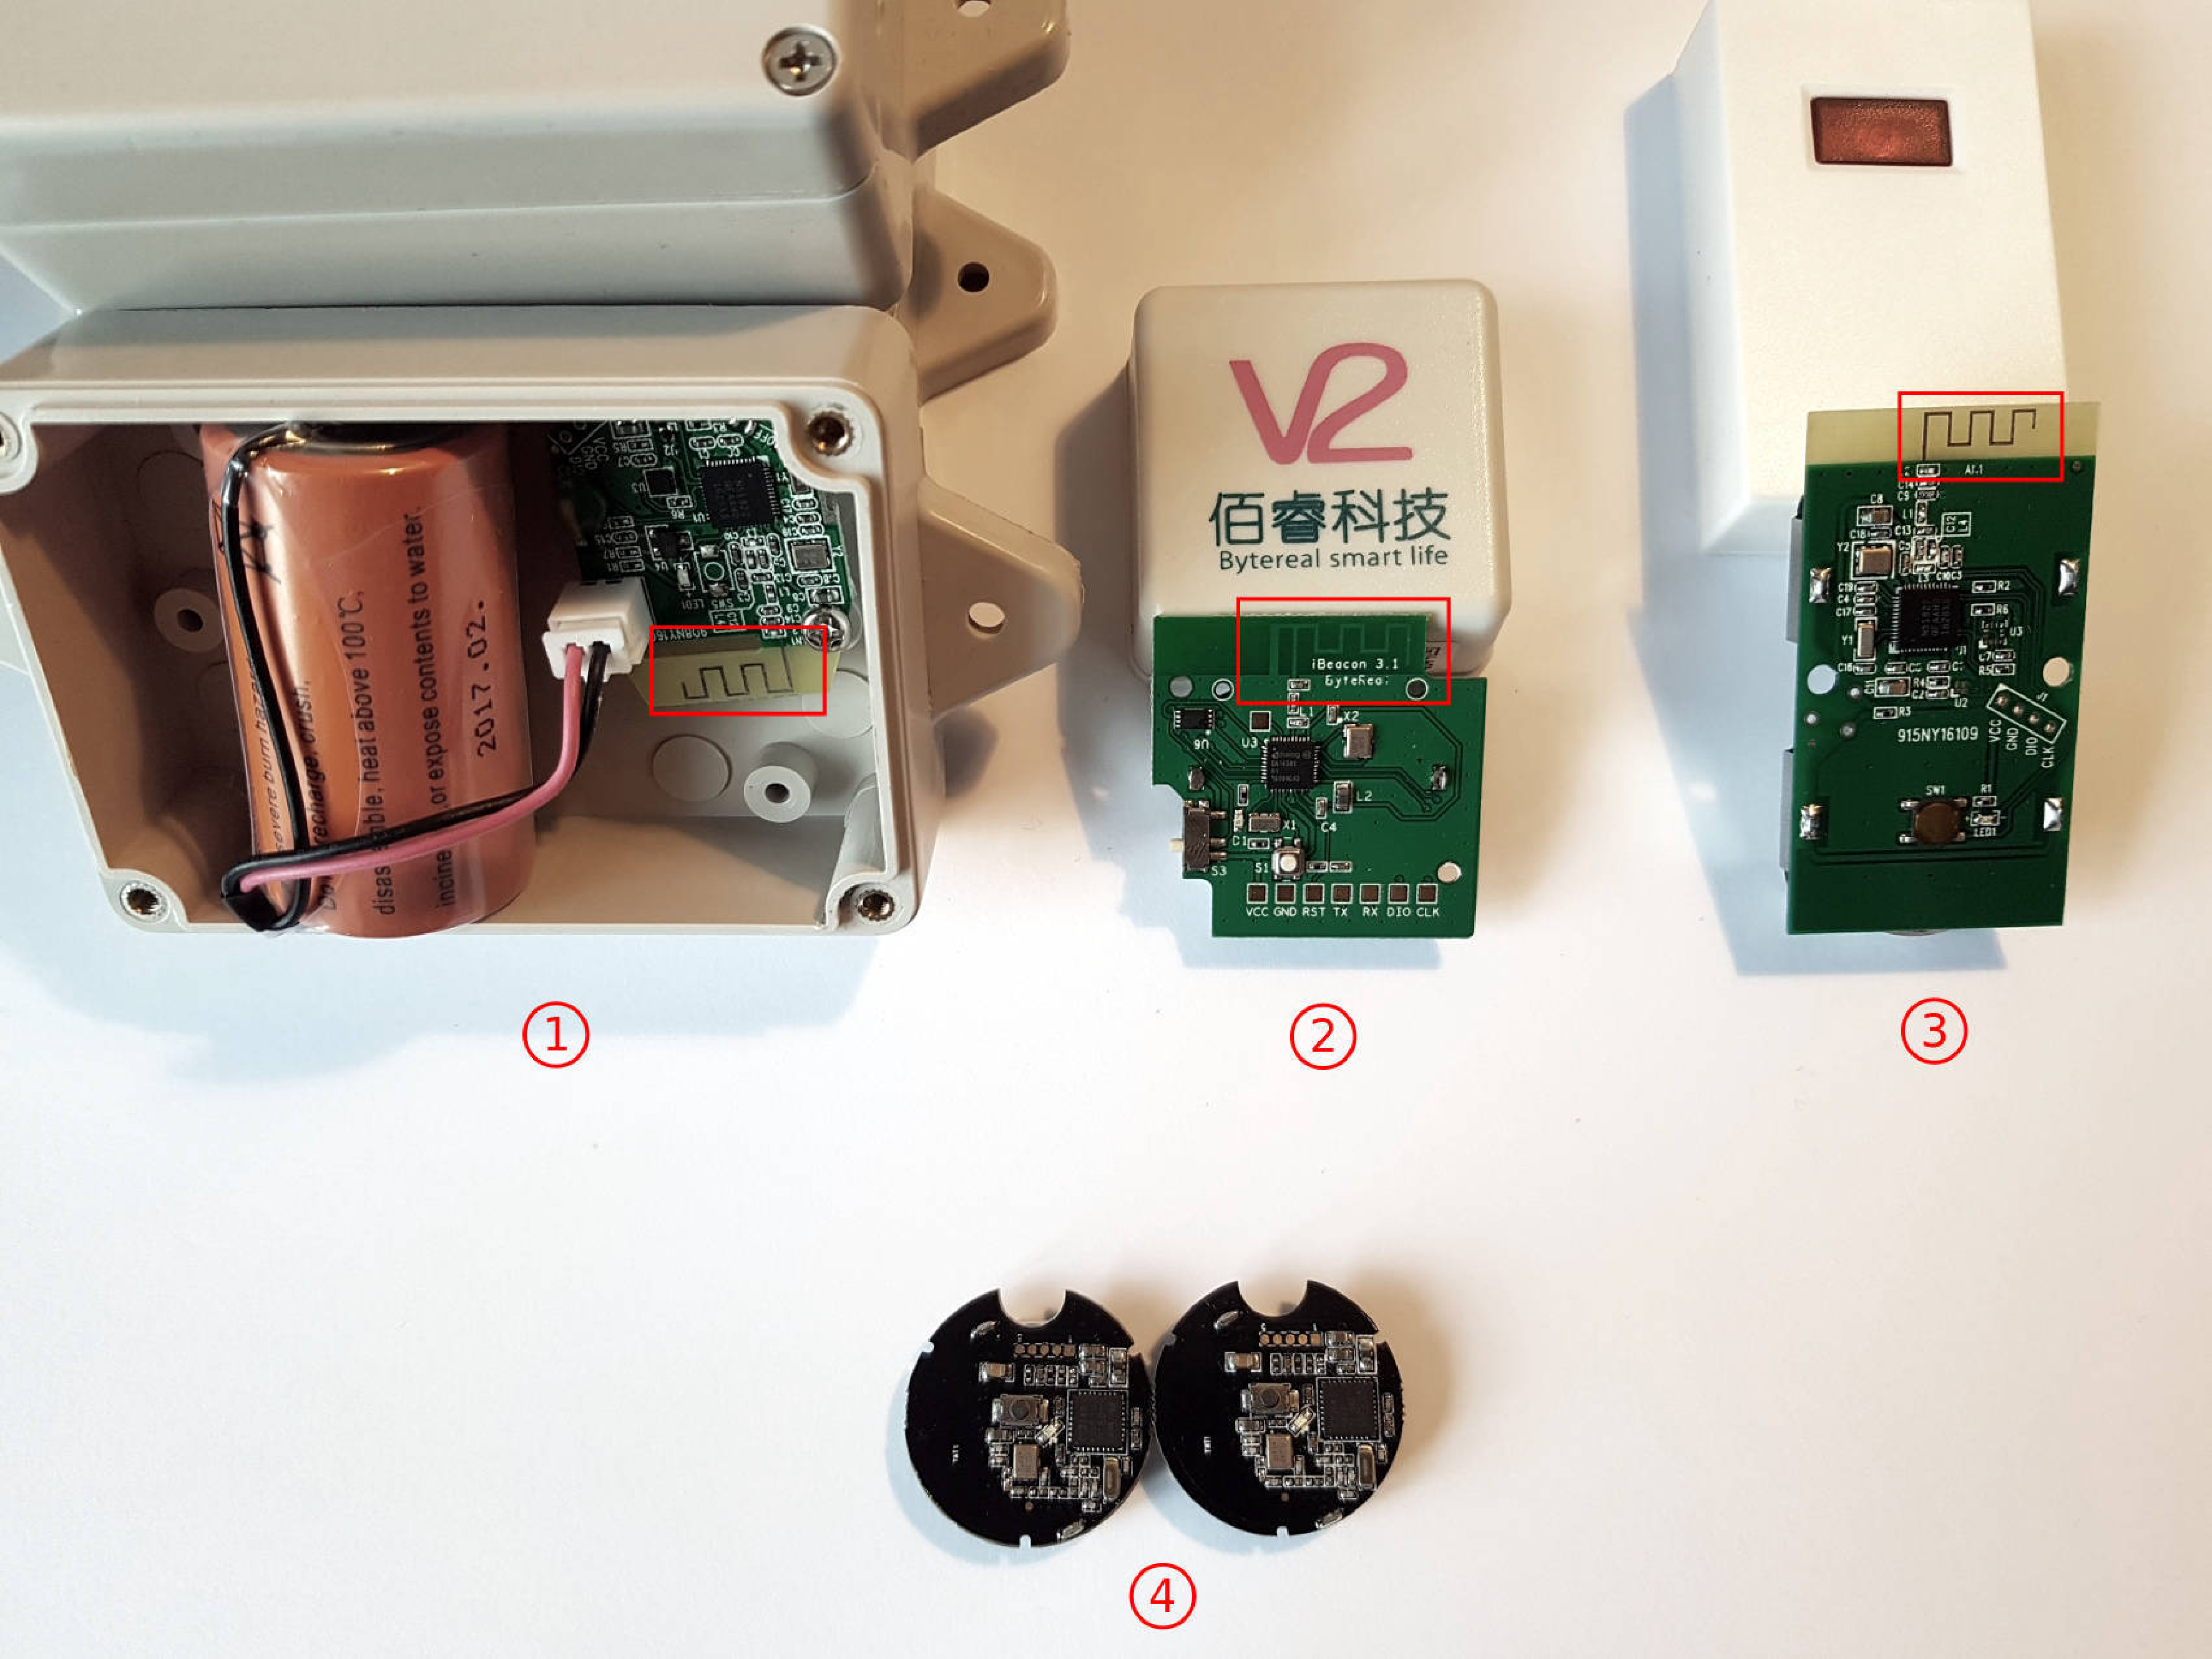
\includegraphics[width=\textwidth, keepaspectratio]{pictures/beacons_used_in_tests.pdf}
\centering
\caption{Beacons transmitters used during tests. Beacon 1 is a Wellcore procduct based on Nordic NRF51822 chip, Beacon 2 is a ByteReal product based on Dialog Semiconductor DA14580 chip, Beacon 3 is a Wellcore product based on Nordic NRF51822 chip, Beacon 4 is a Radioland product based on Texas Instruments TI2640 chip. On pictures there are highlighted antennas placement.}
\label{fig:beacons_used_in_tests}
\end{figure}

TODO: https://superuser.com/questions/805935/how-to-directinize-bluetooth-signal

Hardware tests were designed in a manner that each of those factors were tested separately. There were performed following test cases:

\begin{itemize}
	\item Obtain signal attenuation curve with respect of the power of the transmitter by measuring the received signal stregth at given distances from the signal source.
	\item Signal range per given transmitter power setting and receiver in „pocket” orientation. Dynamic tests in a sequence: * 5 sec under the transmitter, * move 5 meters away (actor is an obstacle), * 5 sec on 5 meters distance

% case 1. There were selected two transmitter power settings for this test case.P ower density measured on discrete distances from signal source
* -12dBm transmitter power
* -16dBm transmitter power
* -20dBm transmitter power
* -30dBm transmitter power
Singal range per given transmitter power setting and different receiver orientation. Static test: directly under the transmitter
* -12dBm transmitter power; orientation: -
* -12dBm transmitter power; orientation: |
* -12dBm transmitter power; orientation: P
* -16dBm transmitter power; orientation: -
* -16dBm transmitter power; orientation: |
* -16dBm transmitter power; orientation: P
* -20dBm transmitter power; orientation: -
* -20dBm transmitter power; orientation: |
* -20dBm transmitter power; orientation: P
* -30dBm transmitter power; orientation: -
* -30dBm transmitter power; orientation: |
* -30dBm transmitter power; orientation: P
Line of sight (LOS) test. Tests performed with no LOS condition. Rest parameters same as in test 1,1. Test is designed to be compared with results of analogue test no. 1,1
* With LOS (source not shadowed, same as 1.1)
* Without LOS (source not visible due to corridor shape)
Impact of actor position; obtain attenuation curve in case where an actor is an obstacle between transmitter and receiver
* 4dBm transmitter power; power density measured on discrete distances from signal source
* 4dBm transmitter power; power density measured on discrete distances from signal source; actor in an obstacle
Obtain transmitter signal attenuation curve per different transmitter antenna directions for transmitter mounted on ceiling
↓direction
→direction
Obtain transmitter signal attenuation curve per different transmitter antenna directions for transmitter mounted on wall
↓direction
→direction
Obtain transmitter signal attenuation curve for different transmitters microcontrollers and hardware
* B1
* B2  - default transmitter power (not changed for tests)
* B3 – was set to -8dBm, but result was observable like -16dBm in B1
* B4
Obtain transmitter signal attenuation curve for different reicevers (smartphones)
* Samsung Galaxy S7 (BLE 4.1)
* Blackberry Z10 (BLE 4.0)
Dynamic tests with 3 beacons. Tested two distances between beacons. Tests start with 5s measurement of signal strength 20m before first transmitter, consists of walk along corridor (70/80m), ends with 5s measurement of signal strength 20m after last transmitter
* transmitter in 10m intervals (two tests: there + way back)
* transmitter in 15m intervals (two test: there + way backs)
Dynamic tests with 3 beacons. Tested two orientations of receiver. Tests start with 5s measurement of signal strength 20m before first transmitter, consists of walk along corridor (70m), ends with 5s measurement of signal strength 20m after last transmitter
* F-/B- (due to movement) receiver orientation
* P receiver orientation
Wall and ceiling transmitter placement comparison
* transmitter on the ceiling
* transmitter on the wall

\end{itemize}

\begin{itemize}
	\item Define factors that are important to state if solution is good or not
	\item Will allow to check if system fulfills requirements
	\item Test features stated in 'Localization system choise section'
\end{itemize}

% section tests_criteria_and_assumptions (end)

\section{Tests metodology} % (fold)
\label{sec:tests_metodology}

\begin{itemize}
	\item Testing environment descipription
	\item Equimpent used during tests. Example:
	\begin{itemize}
		\item using a representative wifi router, 801.11g techonology, simple circular antenna (eg Minetronics MMG) - for charts.
		\item using a representative beacon
		\item dBm signal strength depending on the distance and polarity of the mobile device from the signal source
	\end{itemize}
	\item Pictures
\end{itemize}

% section tests_metodology (end)

\section{Tests of system and basic algorithm} % (fold)
\label{sec:tests_of_system_and_basic_algorithm}
\begin{itemize}
	\item Check if system works with basic algorithm
	\item Tests in few configurations
	\item State if some factors have impact on signal quality
	\item State if some factors have impact on position finding
\end{itemize}
% section tests_of_system_and_basic_algorithm (end)

\section{Tests of extended algorithm} % (fold)
\label{sec:tests_of_extended_algorithm}

Capture data that will be base for comparison between simple and extended position finding algorithm accuracy.

% section tests_of_extended_algorithm (end)

\section{Experiments results} % (fold)
\label{sec:experiments_results}

Resluts with analysis.

% section experiments_results (end)

\section{Tests summary} % (fold)
\label{sec:tests_summary}

% section tests_summary (end)
\end{document}
